% Chapter Template

\chapter{Literature Survey of the VAD algorithms} % Main chapter title

\label{Chapter2} % Change X to a consecutive number; for referencing this chapter elsewhere, use \ref{ChapterX}

\lhead{Chapter 2. \emph{Literature Survey of the VAD algorithms}} % Change X to a consecutive number; this is for the header on each page - perhaps a shortened title

%----------------------------------------------------------------------------------------
%	SECTION 1 - Standard VAD algorithms
%----------------------------------------------------------------------------------------

\section{Standard VAD algorithms}

Being an important tool in many speech processing applications, a number of VAD algorithms have been subject to standardisation by various organisations such as the International Telecommunication Union (ITU-T), European Telecommunications Standards Institute (ETSI), Telecommunications Industry Association (TIA) or Electronic Industries Alliance (EIA). It is important to note that most of the standardised VAD approaches have been developed for use in the telecommunications industry, with particular emphasis on the application for discontinuous transmission (DTX), which may make them less appropriate for other speech processing tasks such as speech recognition.

In the rest of this chapter, three standard VAD algorithms are going to be described:
\begin{itemize}
\item ITU-T G.729 Annex B \citep{G729} which is an extension to the G.729 speech coder with an aim to achieve an improved bit rate during the noise-only periods
\item ETSI AMR1 and AMR2 \cite{AMR} for application to the Global System for Mobile Communications (GSM)
\item TIA/EIA IS-733 \cite{IS733} for application to the Wideband Spread Spectrum Communication Systems
\end{itemize}

\subsection{ITU-T G.729 Annex B}

The well-known ITU-T G.729 Annex B VAD has been developed as an extension to the G.729 speech coding algorithm \citep{G729Original} transmitting each frame at a fixed bit rate of 8 kb/s. Application of the Voice Activity Detector allows to identify the noise-only frames in a continuous stream of data and adopt a compressed transmission at only 15 b/frame which contains information about the background noise for reproduction by the Comfort Noise Generator (CNG) at the receiving end. This approach for speech/noise coding allows to reduce the average bit-rate of the entire coder from 8 kb/s to only 4 kb/s while keeping the transmission quality unchanged.

The block diagram of the VAD algorithm is presented in Figure \ref{fig:G729AnnexB}. It starts with computation of four main \emph{instantaneous parameters} for the current frame which describe the energy and spectral content of the signal:
\begin{itemize}
\item Set of Line Spectral Frequencies (LSF)
\item Full-band energy ($E_f$)
\item Low-band (0 to 1 kHz) energy ($E_l$)
\item Zero-crossing rate (ZCR)
\end{itemize}

\begin{figure}[htbp]
	\centering
		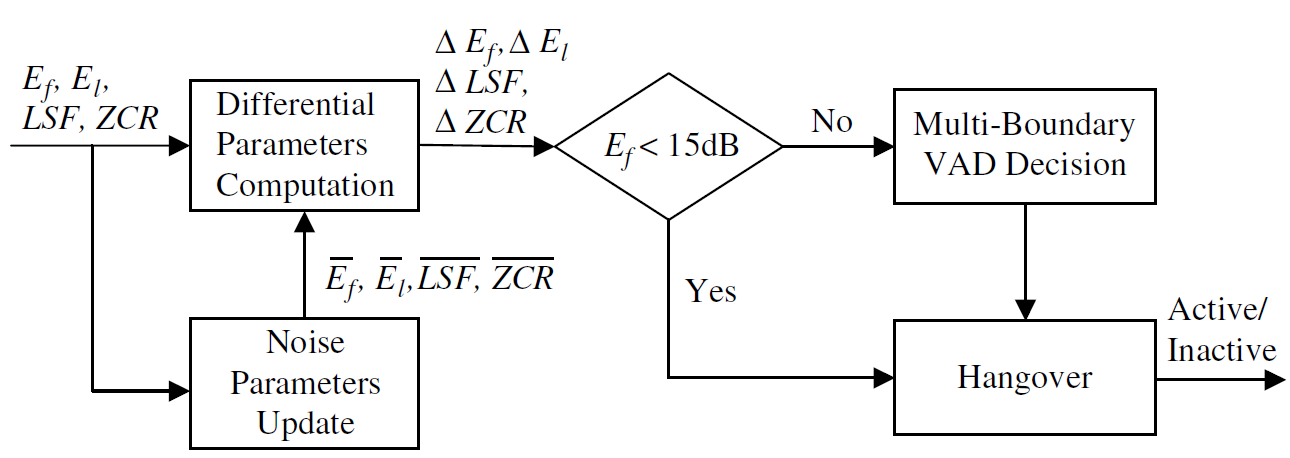
\includegraphics[width=0.9\columnwidth]{Figures/G729AnnexB.png}
		\rule{37em}{0.5pt}
	\caption[Block diagram of the ITU-T G.729 Annex B Voice Activity Detector]{Block diagram of the ITU-T G.729 Annex B Voice Activity Detector \cite{Kondoz}}
	\label{fig:G729AnnexB}
\end{figure}

The \emph{instantaneous parameters} are then differenced with their most recent average noise-only counterparts in order to derive an additional set of so called \emph{difference parameters} which are used for speech/non-speech classification. The set of all possible \emph{difference parameters} describes a four dimensional Euclidean space in which a specific region contains the speech frames while another region describes the noise-only frames. The current vector of parameters is compared against the pre-computed regions in order to classify the current frame. The two regions are initially identified by visual inspection of the points' distribution over a large set of clean and noisy recordings. An energy threshold of $E_f < 15 dB$ is applied before the multi-boundary classification in order to minimise short glitches on low-energy frames.

ITU-T G.729 Annex B uses an additional four-step heuristic-based smoothing scheme after the initial multi-boundary classification:
\begin{enumerate}
\item An active voice decision is extended to the current frame if its energy is above a certain threshold
\item An active voice decision is extended to the current frame if the previous two frames were speech and the absolute energy difference between the current and previous frames' is under a certain threshold
\item An inactive voice decision is extended to the current frame if the previous 10 frames were noise-only and the absolute energy difference between current and previous frames' is under a certain threshold
\item The active voice frame is labelled as inactive if the current frame energy is below a noise floor by a certain threshold
\end{enumerate}

The VAD algorithm also performs updates of the noise parameters ($\overline{LSF}$, $\overline{E_f}$, $\overline{E_l}$ , $\overline{ZCR}$) by a secondary VAD decision which does not need to be extremely robust since it is used only for noise parameters estimation.

\subsection{ETSI AMR1 and AMR2}

ETSI proposed two VAD alternatives for use in the Adaptive Multi-Rate speech traffic channels. In both algorithms, the decision is primarily based on the energy of the signal to be classified across different frequency bands.

The block diagram of the AMR Option 1 VAD is presented in Figure \ref{fig:AMR1}. The input signal is first passed through a series of band-pass filters which split the time-domain signal into different frequency bands based on the Table \ref{AMR1filterbank}.

\begin{table}[htbp]
\center
\begin{tabular}{c|c|}
\cline{2-2}
 & Frequencies \\ \hline
\multicolumn{1}{ |c| }{Bank 1} & 0 - 250 Hz \\ \hline
\multicolumn{1}{ |c| }{Bank 2} & 250 - 500 Hz \\ \hline
\multicolumn{1}{ |c| }{Bank 3} & 500 - 750 Hz \\ \hline
\multicolumn{1}{ |c| }{Bank 4} & 750 - 1000 Hz \\ \hline
\multicolumn{1}{ |c| }{Bank 5} & 1000 - 1500 Hz \\ \hline
\multicolumn{1}{ |c| }{Bank 6} & 1500 - 2000 Hz \\ \hline
\multicolumn{1}{ |c| }{Bank 7} & 2000 - 2500 Hz \\ \hline
\multicolumn{1}{ |c| }{Bank 8} & 2500 - 3000 Hz \\ \hline
\multicolumn{1}{ |c| }{Bank 9} & 3000 - 4000 Hz \\ \hline
\end{tabular}
\caption[Cut-off frequencies for the ETSI AMR1 band-pass filters]{Cut-off frequencies for the ETSI AMR1 band-pass filters \citep{AMR}}
\label{AMR1filterbank}
\end{table}

\begin{figure}[htbp]
	\centering
		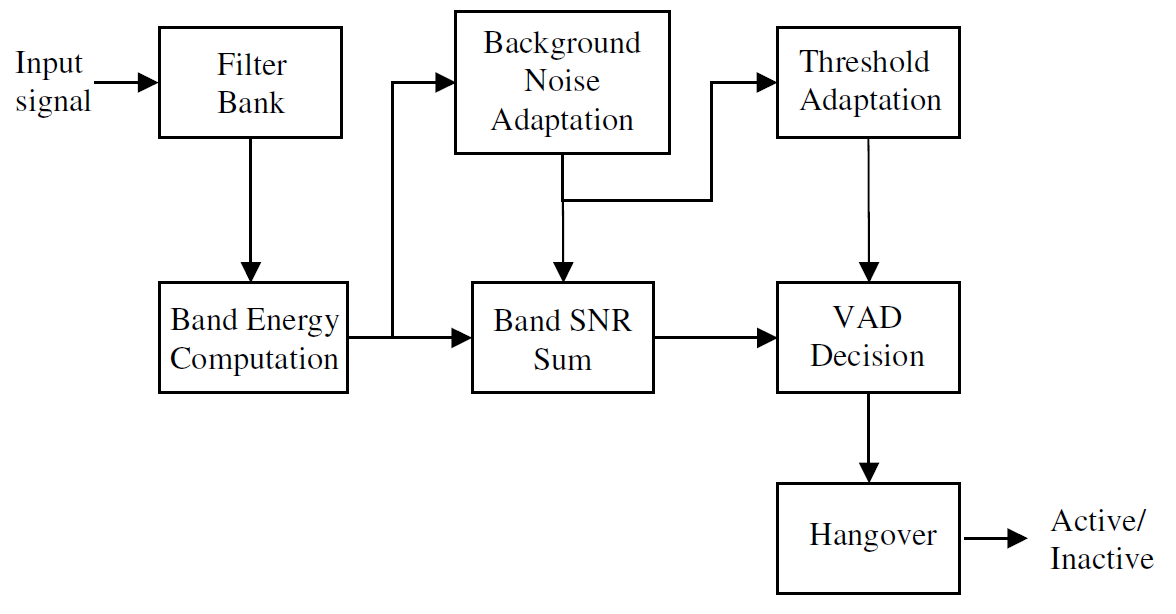
\includegraphics[width=0.9\columnwidth]{Figures/AMR1.png}
		\rule{37em}{0.5pt}
	\caption[Block diagram of the ETSI AMR Option 1 Voice Activity Detector]{Block diagram of the ETSI AMR Option 1 Voice Activity Detector \cite{Kondoz}}
	\label{fig:AMR1}
\end{figure}



%\begin{figure}[htbp]
%	\centering
%		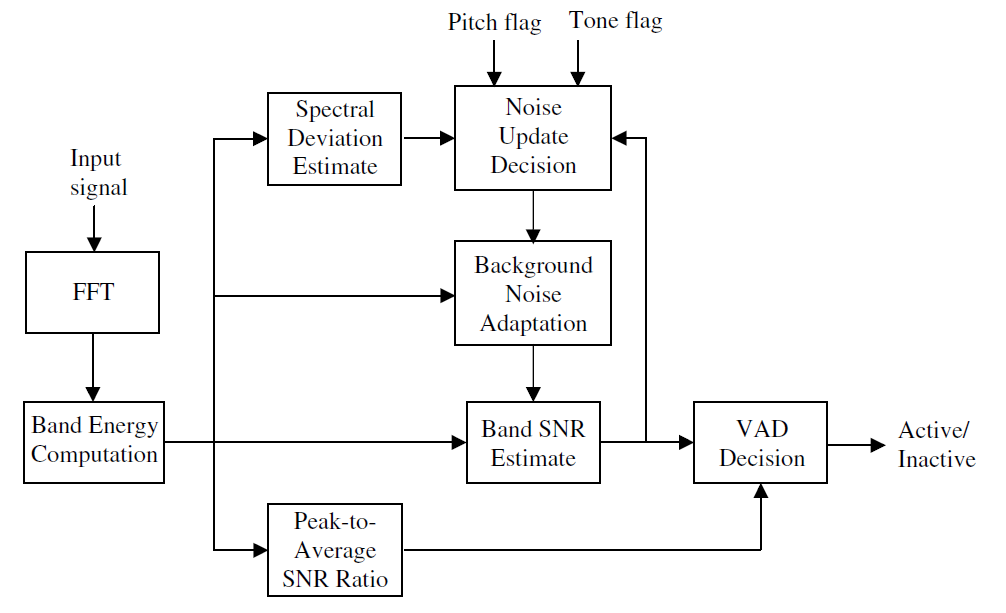
\includegraphics[width=0.9\columnwidth]{Figures/AMR2.png}
%		\rule{37em}{0.5pt}
%	\caption[Block diagram of the ETSI AMR Option 2 Voice Activity Detector]{Block diagram of the ETSI AMR Option 2 Voice Activity Detector \cite{Kondoz}}
%	\label{fig:AMR2}
%\end{figure}

\subsection{TIA/EIA IS-733}

%----------------------------------------------------------------------------------------
%	SECTION 2 - Other VAD algorithms
%----------------------------------------------------------------------------------------

\section{Other VAD algorithms}